\documentclass{beamer}

\newcommand{\course}{CS 1331 Introduction to Object Oriented Programming}
\newcommand{\lesson}{Programming with Exceptions}
\newcommand{\code}{http://www.cc.gatech.edu/~simpkins/teaching/gatech/cs1331/code}

\author[Chris Simpkins] 
{Christopher Simpkins \\\texttt{chris.simpkins@gatech.edu}}
\institute[Georgia Tech] % (optional, but mostly needed)

\date[CS 1331]{}


\newcommand{\course}{Introduction to Object-Oriented Programming}
\subject{\course}
\title[\lesson]{\course}
\subtitle{\lesson}

\author[CS 1331]
{Christopher Simpkins \\\texttt{chris.simpkins@gatech.edu}}
\institute[Georgia Tech]

\date[]{}

\newcommand{\link}[2]{\href{#1}{\textcolor{blue}{\underline{#2}}}}
\newcommand{\code}{http://www.cs1331.org/code}

\usepackage{colortbl}

% If you have a file called "university-logo-filename.xxx", where xxx
% is a graphic format that can be processed by latex or pdflatex,
% resp., then you can add a logo as follows:

% \pgfdeclareimage[width=0.6in]{coc-logo}{cc_2012_logo}
% \logo{\pgfuseimage{coc-logo}}

\mode<presentation>
{
  \usetheme{Berlin}
  \useoutertheme{infolines}

  % or ...

 \setbeamercovered{transparent}
  % or whatever (possibly just delete it)
}

\usepackage{tikz}
% Optional PGF libraries
\usepackage{pgflibraryarrows}
\usepackage{pgflibrarysnakes}
\usepackage{pgfplots}
\usepackage{fancybox}
\usepackage{listings}
\usepackage{hyperref}
\hypersetup{colorlinks=true,urlcolor=blue}
\usepackage[english]{babel}
% or whatever

\usepackage[latin1]{inputenc}
% or whatever

\usepackage{times}
\usepackage[T1]{fontenc}
% Or whatever. Note that the encoding and the font should match. If T1
% does not look nice, try deleting the line with the fontenc.


\usepackage{listings}

% "define" Scala
\lstdefinelanguage{scala}{
  morekeywords={abstract,case,catch,class,def,%
    do,else,extends,false,final,finally,%
    for,if,implicit,import,match,mixin,%
    new,null,object,override,package,%
    private,protected,requires,return,sealed,%
    super,this,throw,trait,true,try,%
    type,val,var,while,with,yield},
  otherkeywords={=>,<-,<\%,<:,>:,\#,@},
  sensitive=true,
  morecomment=[l]{//},
  morecomment=[n]{/*}{*/},
  morestring=[b]",
  morestring=[b]',
  morestring=[b]""",
}

\usepackage{color}
\definecolor{dkgreen}{rgb}{0,0.6,0}
\definecolor{gray}{rgb}{0.5,0.5,0.5}
\definecolor{mauve}{rgb}{0.58,0,0.82}

% Default settings for code listings
\lstset{frame=tb,
  language=scala,
  aboveskip=2mm,
  belowskip=2mm,
  showstringspaces=false,
  columns=flexible,
  basicstyle={\scriptsize\ttfamily},
  numbers=none,
  numberstyle=\tiny\color{gray},
  keywordstyle=\color{blue},
  commentstyle=\color{dkgreen},
  stringstyle=\color{mauve},
  frame=single,
  breaklines=true,
  breakatwhitespace=true,
  keepspaces=true
  %tabsize=3
}


% If you wish to uncover everything in a step-wise fashion, uncomment
% the following command: 

% \beamerdefaultoverlayspecification{<+->}


\begin{document}

\begin{frame}
  \titlepage
\end{frame}


%------------------------------------------------------------------------
\begin{frame}[fragile]{Programming with Exceptions}

\begin{itemize}
\item Understanding Java's exception class hierarchy
\item Understanding how exceptions work
\item Principles for programming with exceptions
\item Writing and using your own exception classes
\end{itemize}

\end{frame}
%------------------------------------------------------------------------

%------------------------------------------------------------------------
\begin{frame}[fragile]{Java's Exception Hierarchy}

\begin{columns}[t]
\begin{column}{2in}
\begin{center}
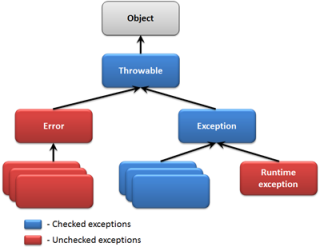
\includegraphics[height=2.5in]{hierarchy_of_java_exceptions.png}
\end{center}
\end{column}
\begin{column}{3in}
\begin{itemize}
\item Most (checked) exceptions will subclass {\tt Exception}
\item Most uncheked exceptions will subclass {\tt RuntimeException}
\item {\tt Error} is for compiler hackers.  Don't use it directly.
\end{itemize}
\end{column}
\end{columns}

\end{frame}
%------------------------------------------------------------------------


%------------------------------------------------------------------------
\begin{frame}[fragile]{Throwing Exceptions is a Control Flow Mechanism}


What does this code print?
\begin{lstlisting}[language=Java]
public class Wee {

    static void bar() throws Throwable {
        throw new Throwable("Wee!");
    }

    static void foo() throws Throwable {
        bar();
        System.out.println("Foo!");
    }

    public static void main(String[] args) {
        try {        
            foo();
        } catch (Throwable t) {
            System.out.println(t.getMessage());
        }
        System.out.println("I'm still running.");
    }
}
\end{lstlisting}

\end{frame}
%------------------------------------------------------------------------

%------------------------------------------------------------------------
\begin{frame}[fragile]{Principles of Exception Handling}


\begin{itemize}
\item Don't try to handle coding errors.
\item Prefer exceptions from the standard library to creating your own.
\item Name exceptions after the problem (not the thrower).
\item Wrap exceptions when crossing an abstraction boundary.
\item Store useful information in exception objects.
\item Handle exceptions close to their origins, but ...
\begin{itemize}
  \item Assign exception-handling responsibility to objects that can handle the exceptions.
  \item Don't ``eat'' exceptions (at the very least, log the exception).
  \item If you can't handle an excepotin sensibly, propagate it (``when in doubt, throw it out'').
\end{itemize}
\end{itemize}

See \url{http://wirfs-brock.com/PDFs/towards_xcptn_hndling.pdf} for more details.  We'll just touch on a few of these here.

\end{frame}
%------------------------------------------------------------------------

%------------------------------------------------------------------------
\begin{frame}[fragile]{Applying Exception Handling Principles}


What's wrong with this constructor?
\begin{lstlisting}[language=Java]
public class Company {
    private ArrayList<Employee> employees;

    public Company(String employeeDataFile) {
        employees = new ArrayList<Employee>(10);
        try {
            initFromFile(new File(employeeDataFile));
        } catch (FileNotFoundException e) {
            System.out.println("Employee data file not found.");
        } catch (ParseException e) {
            System.out.println("Malformed data file: "+e.getMessage();
        } catch (Exception e) {
            System.out.println("Exception occurred: "+e.getMessage());
        }
    }
    //...
}
\end{lstlisting}

\end{frame}
%------------------------------------------------------------------------

%------------------------------------------------------------------------
\begin{frame}[fragile]{Writing and Using Your Own Exceptions}


Define your own exception classes by subclassing {\tt Exception} (for checked exceptions) or {\tt RuntimeException} (for unchecked exceptions). 

\begin{lstlisting}[language=Java]
public class MyException extends Exception {

    public MyException(String msg) {
        super(msg);
    }
}
\end{lstlisting}
And use them just like any other exception:
\begin{lstlisting}[language=Java]
if (checkProblem()) {
    throw new MyException("Oops!");
}
\end{lstlisting}

But remember: in most cases there is an Exception class in the standard library that you can use. Don't write your own exception classes unless you really need to.

\end{frame}
%------------------------------------------------------------------------

%------------------------------------------------------------------------
\begin{frame}[fragile]{Use The Most Specific Applicable Exception}


Recall our {\tt Company} constructor:
\begin{lstlisting}[language=Java]
try {
    initFromFile(new File(employeeDataFile));
} catch (FileNotFoundException e) {
    //...
} catch (ParseException e) {
    //...
} catch (Exception e) {
    //...
}
\end{lstlisting}
With separate exceptions we can take more specific actions, e.g.:
\begin{itemize}
\item We can tell the user to check for the right file (FileNotFoundException).
\item We can tell the user that the data file is malformed (ParseException).
\end{itemize}


\end{frame}
%------------------------------------------------------------------------

%------------------------------------------------------------------------
\begin{frame}[fragile]{Final Thoughts}

\begin{itemize}
\item Use exceptions for their intended purpose: separating your core logic from the code that handles exceptional conditions.
\item Use exceptions judiciously (not too many).
\item Think about how you handle exceptions:
\begin{itemize}
\item have sound reasons for propagating exceptions you propagate
\item have sound reasons for catching exceptions where you catch them
\item recover if you can
\item store information in your exceptions to aid in debugging or error recovery by the user
\end{itemize}
\end{itemize}


\end{frame}
%------------------------------------------------------------------------

% %------------------------------------------------------------------------
% \begin{frame}[fragile]{}


% \begin{lstlisting}[language=Java]

% \end{lstlisting}

% \begin{itemize}
% \item
% \end{itemize}


% \end{frame}
% %------------------------------------------------------------------------


\end{document}
